\chapter{Methodology}
\label{chap:methodology}

In this chapter, we will cover the methodology used in this work. More details on the pipeline execution will be provided in Section \ref{sec:backend}.

\section{Prediction Using the CryptoBench Model, ESM-2}
\label{sec:prediction}

The initial step in our methodology involves utilizing the CryptoBench \cite{vskrhak2025cryptobench} model to generate residue-level predictions for protein sequences. It is important to note that this model works solely with sequence information, without incorporating any structural (tertiary or quaternary) data. Specifically, we employ the tiny variant of CryptoBench\footnote{Available at \url{https://github.com/skrhakv/TinyCryptobench}}, which is trained on a reduced version of the fine-tuned ESM-2 embeddings \cite{lin2022language} with 650 million parameters, as opposed to the full 3 billion. This choice is motivated by the observation that prediction accuracy remains comparable, while computational requirements are significantly reduced, enabling the pipeline to run efficiently on standard personal computers without the need for a GPU.

CryptoBench was created by filtering the AHoJ-DB \cite{feidakis2024ahoj} dataset, which contains a few million binding pockets. The filtering steps involved resolution filtering, removing redundant structures, geometric quality assurance, crypticity constraints, ligand filtering and sequence clustering. The final dataset consists of 1107 apo structures with 1361 cryptic binding sites. This dataset is used to train the model that has been benchmarked against PocketMiner \cite{meller2023predicting} and P2Rank \cite{krivak2018p2rank} and has shown better performance with the apo structures.

\sloppy
To begin with the prediction, the necessary dependencies for the CryptoBench model must be installed. Once the Python environment is set up, the fine-tuned ESM-2 model (\lstinline!facebook/esm2_t33_650M_UR50D!) is loaded, followed by the corresponding weight file from the Tiny-CryptoBench repository. The protein sequence is then tokenized using the ESM-2 tokenizer, segmented into chunks of 1022 tokens (1024 minus two special tokens), and processed by the CryptoBench model to obtain predictions. These predictions are subsequently concatenated to produce a single prediction vector representing the entire sequence.

\sloppy
The implementation for this procedure is provided in the \lstinline!backend/prediction/compute_score.py! file. The code is intended for use with individual protein sequences, as it requires parsing and splitting the sequence by chain to ensure accurate predictions.

This code is run asynchronously using Celery workers, allowing efficient processing of multiple sequences in parallel. Moreover, the implementation supports both GPU and CPU execution.

After the predictions are generated, the next step is to look for potential clusters of high-scoring residues and create the corresponding binding site candidates, as described in Section~\ref{sec:clustering}.

\section{Clustering and Smoothing}
\label{sec:clustering}

The next step in our methodology is to take the residue-level predictions generated by the CryptoBench model and cluster the high-scoring residues to form potential binding site candidates. This is crucial for the visualization as coloring the clusters instead of just individual residues increases the interpretability of the results. The clustering process is based on the 3D coordinates of individual residues, which are obtained from the given structure file.

The clustering process is implemented in the \lstinline!backend/clustering! dictionary. There are many algorithms available for clustering, namely DBSCAN \cite{schubert2017dbscan}, single-linkage clustering, hierarchical clustering \cite{jarman2020hierarchical}, and many more. In our case, we opted for the DBSCAN algorithm, which is a density-based clustering algorithm that groups together points that are closely packed together. This approach is particularly suitable for our use case, as it allows us to identify clusters of high-scoring residues without requiring a predefined number of clusters, and allows the specification of minimum residue distance and minimum number of residues in a cluster.

Our method relies on three parameters to control the clustering process:
\begin{itemize}
    \item \textbf{EPS ($\epsilon$)} - This parameter defines the maximum distance between two residues for them to be considered as part of the same cluster. In our case, we opted for a value of \textbf{5.0 \AA}, which is a reasonable distance for residues when considering their spatial proximity in a protein structure.
    \item \textbf{Minimum cluster size} - This parameter defines the minimum number of residues required to form a cluster. We set this value to \textbf{3}, as 2 residues are not sufficient to form a binding site candidate.
    \item \textbf{Minimum (CryptoBench) prediction score} - This parameter defines the minimum score a residue must have to be marked as a high-scoring residue. We opted for a value of \textbf{0.7}, which covers most cryptic binding sites in the CryptoBench dataset, while also not marking the entire protein as a binding site candidate.
\end{itemize}

The values for these parameters were chosen arbitrarily based on previous experience and benchmarks (covered in this section below). However, these parameters can be adjusted to suit the specific needs. In the implementation, the \textbf{scikit-learn} implementation of the DBSCAN algorithm is used. The clustering works with two method parameters, the 3D coordinates of the residues and the CryptoBench prediction scores.

After the clustering is performed, it seems like the task is done, but there are still some steps to perform. The first problem is to know if the method performs well, i.e. if the clusters correspond to actual binding sites. To address this, we have created a benchmarking notebook that allows us to visualize interesting metrics. We will compare the clusters with the known binding sites from the CryptoBench test set, which contains a few hundred cryptic binding sites. The benchmarking notebooks and other source codes are available in the \lstinline!cryptoshow-benchmark! directory. Note that:

\begin{itemize}
    \item The benchmarking is performed on the CryptoBench test set, not the tiny variant used in the pipeline. This might lead to slightly different results, but the overall performance should be similar.
    \item Multi-chain pockets are omitted from the benchmarking, as the process would be much more complicated and the prediction would require complex approaches.
    \item Many cryptic binding sites in the test set are similar to each other, which can lead to heavily inflated results. To address this, we have used the \textbf{Szymkiewicz–Simpson coefficient (overlap)}, which is a measure of similarity between two sets $A, B$ defined as:
    \begin{equation}
        \text{Szymkiewicz–Simpson}(A, B) = \frac{|A \cap B|}{\min(|A|, |B|)}
    \end{equation}
    After computing the overlap between each pair of cryptic binding sites in one structure, we keep only the CBSs with the overlaps under 0.5.
\end{itemize}

The benchmarking follows the same procedure as the CryptoShow pipeline - first, the predictions are generated for each of the test set structures, then the clustering is performed with the same parameters as in the pipeline. After creating the clusters, we compute the following metrics for each cluster and compare them with the known binding sites:

\begin{itemize}
    \item \textbf{Distance between the cluster center and the CBS center} - This metric is computed as the distance between the cluster center and the center of the cryptic binding site. Both centers are computed as the average of the 3D coordinates of the residues in the cluster and the CBS, respectively. The distance is computed in \AA.
    \item \textbf{Percentage of CBS residues covered by the cluster} - This metric is computed as the percentage of residues in the CBS that are also part of the cluster.
    \item \textbf{Dice coefficient} - This metric is computed as the ratio of the number of residues in the intersection of the cluster and the CBS to the average number of residues in both sets $A, B$. It is defined as:
    \begin{equation}
        \text{Dice}(A, B) = \frac{2 |A \cap B|}{|A| + |B|}
    \end{equation}
\end{itemize}

After computing the metrics for all clusters and one specific CBS, the best-matching cluster is selected based on the top-scoring metric. After doing this for all CBSs and structures, we can see the overall performance of the clustering method. The results are visualized in Figure \ref{fig:clustering-benchmark}.

\begin{figure}[htbp]
    \centering
    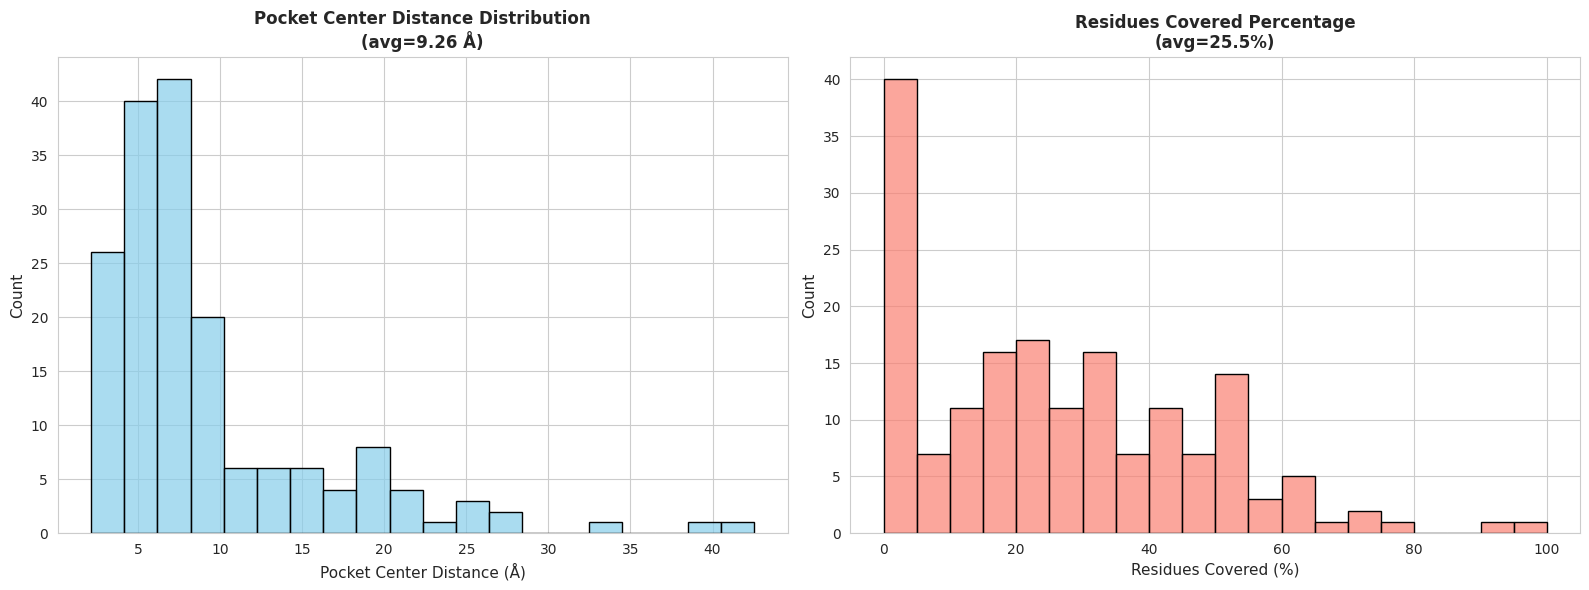
\includegraphics[width=\textwidth]{img/non-smoothened-1.png}
    \caption{Clustering benchmark results. The left plot shows the distance between the cluster center and the CBS center, and the right plot shows percentage of residues covered by the found clusters.}
    \label{fig:clustering-benchmark}
\end{figure}

The results show that the method performs rather poorly, with the average distance between the cluster center and the CBS center being around 10 \AA, and the percentage of CBS residues covered by the cluster being around 25\%. This might not be a bad result as one missing residue in the binding site can lead to a significant increase in the distance, but the percentage of residues covered is rather low. This is caused by the fact that the clustering is performed only on the high-scoring residues. But, some of the CBSs have residues with low scores (supported by Figure \xxx{TODO}), which are still part of the binding site.

What to do next?

\xxx{TODO: add explanation of smoothing, add the training code, some statistics, and the results, then the comparsion with the non-smoothened clustering}
\xxx{TODO: add citations}
\xxx{TODO: potential drawbacks}
\xxx{TODO: reformat}

\section{Trajectory Animation}
\label{sec:trajectory}

\xxx{TODO}
